% -*- mode: latex -*-
\documentclass[12pt,reqno]{amsart}

\usepackage{amsmath}
\usepackage{setspace}
\usepackage[margin=1in]{geometry}
\usepackage{graphicx}
\usepackage{float}
\usepackage{minted}
\usemintedstyle{emacs}

\begin{document}

\newcommand{\pdiff}[2]{\frac{\partial #1}{\partial #2}}
\newcommand{\mytime}{\: \textrm{s}}
\newcommand{\length}{\: \textrm{cm}}
\newcommand{\vel}{\: \frac{\textrm{cm}}{\textrm{s}}}
\newcommand{\mass}{\: \textrm{g}}
\newcommand{\vol}{\: \textrm{cm}^3}
\newcommand{\dens}{\: \frac{\textrm{g}}{\textrm{cm}^3}}
\newcommand{\visc}{\: \frac{\textrm{g}}{\textrm{cm}\cdot\textrm{s}}}
\newcommand{\viscSI}{\: \textrm{Pa}\cdot\textrm{s}}
\newcommand{\abs}[1]{\left| #1 \right|}

%====================
% Equations
%====================

%====================
% Figures
%====================
% fig:generic-oscope
% fig:trigger

%====================
% Tables
%====================

%====================
% Footnotes
%====================
\newcommand{\hickman}{${}^1$}
\newcommand{\nidaq}{${}^2$}
\newcommand{\nobel}{${}^3$}

%====================
% Definitions
%====================
\newcommand{\device}{NI USB-6009}
\newcommand{\progname}{Poscope}
\newcommand{\tdiv}{t_{div}}
\newcommand{\vdiv}{V_{div}}
\newcommand{\sps}{\:\frac{\textrm{samples}}{\textrm{second}}}

\author{Gerrit Slopsema}
\title{PoScope - Software Oscilloscope}
\date{\today}
\begin{abstract}
  We outline the generic structure of oscilloscopes and the particular structure of \progname{}, a software oscilloscope. \progname{}, coupled with the \device{}, acts as an oscilloscope suitable for simple tasks and limited frequency ranges.
\end{abstract}
\maketitle

\section{Introduction}

The oscilloscope was invented in 1897 by Karl Ferdinand Braun\nobel{}. Braun was experimenting with electron beams and found that a screen coated with phosphor illuminates when bombarded with the electrons. From this he made the first cathode ray tube. He applied this to measuring voltage versus time and created the oscilloscope. Braun was awarded a Nobel Prize due to his work in wireless telegraphy.

An oscilloscope is, conceptually, a very simple device. It takes a time-varying voltage input and displays the data as a graph of voltage vs. time. A simplified schematic\hickman{} of a generic oscilloscope can be seen in Figure \ref{fig:generic-oscope}. In this schematic, the voltage input is fed through a voltage attenuator which increases or decreases the voltage to fit the voltage levels to the volts per division setting on the scope.

\begin{figure}[H]
  \begin{center}
    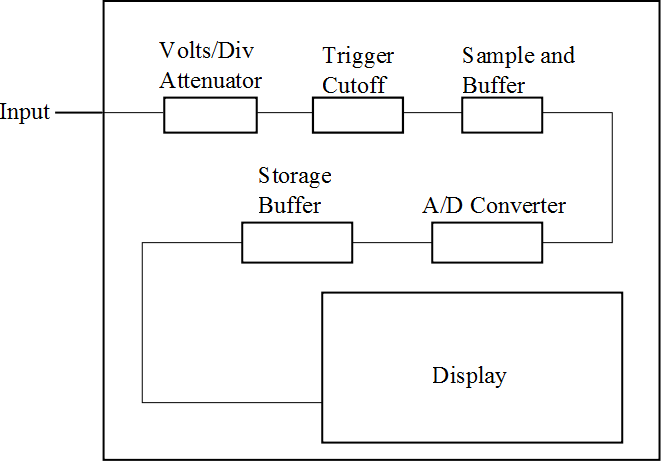
\includegraphics[scale=0.5]{images/generic-oscope.png}
  \end{center}
  \label{fig:generic-oscope}
  \caption{A generic oscilloscope schematic.}
\end{figure}

The data is then routed to the trigger cutoff where the scope reads until a voltage equalling the trigger level is found\hickman{}. There are two methods of triggering: rising slope (or edge) or falling slope (or edge). In the first case the scope searches for the trigger value when the voltage slope is positive. In the second case the scope searches for the trigger value when the voltage slope is negative. The scope only sends the data on after these two conditions (either positive slope and voltage greater than trigger or negative slope and voltage less than trigger) are met. A diagram of this can be seen in Figure \ref{fig:trigger}.

\begin{figure}[H]
  \centering
  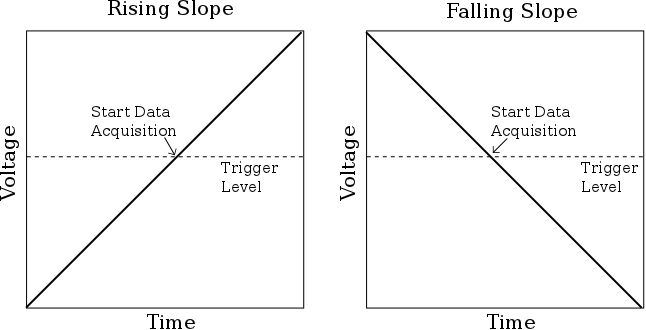
\includegraphics[scale=0.5]{images/trigger.png}
  \caption{Rising and falling slope triggers.}
  \label{fig:trigger}
\end{figure}

After the voltage reaches the trigger level the scope sends the voltage stream to the sampler. The sampler takes the continuous analog voltage signal and \textit{samples} data points from it. For example, in a stream of voltage 500 ms long the sampler may record 1000 voltage levels, each spaced equally in the 500 ms timeframe (reading at a rate of $\frac{500}{1000} = 0.2 \frac{\textrm{samples}}{\textrm{ms}} = 2000 \frac{\textrm{samples}}{\textrm{sec}}$ in this case). The sampler stores these values as a discrete approximation to the continuous voltage stream.

Once the data is obtained the scope can display it on the screen. The scope must accomodate two variables in this display: the volts per division and time per division. In effect, the volts per division dictate how tall the voltage graph appears on the screen. The scope's screen has a fixed number of horizontal lines acting as reference for the voltage levels. Thus the scope must display the data relative to these lines. For example, if the screen has 5 horizontal lines and the volts/div setting is at 1 volt/div, then the maximum voltage difference viewable on the screen is 5 volts. The scope must scale the voltage image according to the size dictated by the volts/div. The same idea applies to the time/div variable, only along the horizontal axis.

\section{Methods}

\subsection{General Structure}
The \progname{} program is a software oscilloscope written in the Python programming language. It uses NI-DAQmx, a software library provided by National Instruments for access to National Instruments devices, NumPy, a scientific computing library, and Qt/Qwt, a library for graphical user interfaces (Qt) and graphical plotting (Qwt).

\progname{} uses a device from National Instruments (\device{}) to read voltage data. A voltage source is connected to the \device{} (with the positive into analog input ``AI0'' and negative into ``GND'') and the \device{} is connected to a computer via USB. \progname{} reads from the \device{}, manipulates the data according to the user's specifications, and displays it on a graph.

\progname{}'s internals differs from Figure \ref{fig:generic-oscope} in the order in which the data is processed. All the steps are present, however the order is as follows:

\begin{enumerate}
\item Voltage is input to the \device{}.
\item The \device{} samples the voltage (sample rate controlled by \progname{}) and converts from analog to digital.
\item \progname{} reads the data from the \device{} into a buffer.
\item \progname{} applies the trigger cutoff.
\item \progname{} manipulates the data to account for scaling, volts/div and time/div, and vertical positioning settings.
\item \progname{} graphs the data on the screen.
\end{enumerate}

The above constitutes one plot cycle.

\subsection{Definitions}
We will use a few variables defined here:

\begin{center}
  \begin{tabular}[H]{c l}
    $n$ & Number of data points graphed per plot cycle. \\
    $r$ & Sample rate of the \device{} (in samples per second). \\
    $\tdiv$ & Time per division (in seconds). \\
    $n_t$ & Number of time divisions on the graph/screen. \\
    $\vdiv$ & Volts per division (in Volts). \\
    $n_V$ & Number of voltage divisions on the graph/screen.
  \end{tabular}
\end{center}

Note that $n/r$ is the time duration of the sample and $n_t\tdiv$ is the time duration displayed on the graph.

\subsection{Triggering}
The \device{} has triggering capabilities\nidaq{} but I was unable to make it work. It is, however, a simple procedure to implement in software. I considered a few triggering methods, some complicated and some easy, and settled on a simple method which works for \textit{most} cases. Assuming the voltage data is periodic and the period of the data is less than $n_t\tdiv$, \progname{} requests $2n$ data points from the \device{}. Once \progname{} has the data, $d = \{d_1, d_2, \dots, d_{2n}\}$, it searches through $d$ until it finds a $d_{i-1}$ and $d_i$ such that $d_{i-1}$ is less than the trigger level and $d_i$ is greater than the trigger level. This is an example of a rising-slope trigger. Once these $d_{i-1}, d_i$ are found \progname{} reads the next $n$ data points from $d$ and uses that as the data to graph. 

Because we assume the period of the data is less than $n_t\tdiv$ we are guaranteed that there are $n$ data points after $d_i$. In the ``worst case'' scenario (with $\tdiv$ set accordingly), the graph will display $n$ data points (that is, $n_t\tdiv = n/r$). However, since the period of the data is less than $n_t\tdiv$, the period is also less than $n/r$. So if the voltage level reaches the trigger level in one period, this ``double-buffer'' method catch the trigger level and have $n$ data points to display on the graph.

\subsection{Vertical Position}
The data read from the \device{} is not always centered around 0. For example, with a sine wave input from a function generator, the recorded voltages may vary from 1 V to -2 V, rather than the desired 1.5 V to -1.5 V. To determine the proper vertical shift required make the voltages symmetric about the horizontal axis, we use the following algorithm:
\begin{minted}[frame=lines,linenos=true]{python}
amplitude = (max(data) - min(data)) / 2
correction = amplitude - max(data)
data = [x + correction for x in data]
\end{minted}
Because the data is periodic, it has a set amplitude. Since we want the data to be centered horizontally around the time-axis, we want the maximum of the data to be at the amplitude. So, line 1 gives the amplitude and line 2 gives the deviation of the maximum from that amplitude, the correction. Then each data point is corrected by adding the correction to it. The result is a shift up or down so that the data is centered around the horizontal axis.

\subsection{Plot Scaling - Time}
The \device{} can sample data at varying rates. The maximum sample rate\nidaq{} is $r_{max} = 48,000 \sps$. Further, the number of samples graphed, $n$, is variable. Both must be considered when determining how much data to use for the plot. Usually some of the data read from the \device{} will be discarded. This is due to the time/div setting. The following algorithm determines the number of data points to use:
\begin{minted}[linenos=true, frame=lines]{python}
# The time duration of the actual data sample 
# = 
# (number of samples) / (sample rate)
time_duration = n / r
# The maximum plottable time 
# =
# (time per division) * (number of time divisions on graph)
time_maximum = t_div * n_t
if time_duration > time_maximum:
    index_maximum = int(time_maximum * r)
else:
    index_maximum = n
plottable_range = data[0:index_maximum]
\end{minted}
Lines 9 - 12 determine the maximum index that can be graphed. This can be explained by considering a dataset $d = \{d_1, d_2, \dots, d_m\}$. If the data is recorded at a rate $r \sps$, then the duration of the read is $m / r$ seconds. However, the graph can show a maximum time duration $t_{max} = \tdiv n_t$ (the time per division times the number of divisions). So, if the time represented by the data is greater than $t_{max}$ (line 9) then we must find the data range within $d$ which can be plotted. The index of this $d_i$ is given by $i = \lfloor t_{max} r \rfloor$. If, however, the time duration of the read is less than $t_{max}$, then we simply display the available data. This will result in a portion of the graph being empty. An improvement on this would be to read more data until $t_{max}$ is met. Thus the plottable data is $d_{plottable} = \{d_1, d_2, \dots, d_i\}$. Line 13 is the pythonic way of taking a range of an array.

\section{Results}
\progname{} is a working example of a software oscilloscope. It accurately displays the waveforms provided it. The performance is adequate, however the framerate of the plot is low. This is due to the time required to sample enough data, process that data, and display it. Using the default settings (timer = 10 ms, $n = 1000$, $r = 10000$) the program will restart the plot cycle every 10 milliseconds, read data for another $2n / r = 20$ milliseconds ($2n$ due to double-buffer triggering), process the data for an indeterminate amount of time, and generate a static plot figure, again using an indeterminate amount of time.

Using a conservative estimate of 20 milliseconds for the time required to process the data and generate the graph, each frame takes a minimum of 40 milliseconds to complete. This leads to a framerate of $1000 / 40 = 25$ frames per second. The plot animation appears relatively smooth at this framerate, however it could stand for improvement.

Both the read times and the processing times can be reduce, however. By reducing $n$, we can reduce both the read time and the processing time. Further, increasing $r$ will reduce the read time, but will also cause the data to represent a shorter time duration. It will, however, give a higher resolution to the data.

The performance of the trigger could be improved by using a \textit{continuous read} rather than a fixed-size read. That is, instead of using double-buffer triggering wherein we read $2n$ datapoints, we could set the \device{} to send a stream of data points. Rather than first reading twice the amount of data necessary, the program could look at each data point individually, compare it to the trigger level, and discard it after use. Only when it found a value greater than the trigger would \progname{} shut off the continuous stream and request $n$ more data points. There would thus be less data storage and, on average, the \device{} would not end up reading all $2n$ data points. The NI-DAQmx interface offers such a function however the \device{} does not support it. This places practical limitations on the device, as certain waveforms or plots may appear choppy.

\section{Conclusion}
The software presented here is an adequate oscilloscope for simple tasks and limited frequency ranges. Its limitations lie in speed of operation, features, and its ability to read data \textit{only} from the \device{}. 

\section{Future Work}
\progname{} can be extended in many areas. The first is functionality. Currently \progname{} supports only 1 input (one channel) however the \device{} has 8 analog inputs and 8 digital inputs. It is therefore possible to have up to 16 channels on the scope. The vast array of options and configurations available on hardware oscilloscopes can also be coded in.

There are many techniques described in Hickman\hickman{} which conventional digital oscilloscopes use to enhance the quality of the samples. Included in these are data smoothing and data averaging, both of which considerably help the discrete samples appear more continuous when graphed and reduce noise. This would allow for a smaller number of samples taken and speed up the data processing and graphing, all of which would speed up the whole program.

The program is written in Python, an easy to use but relatively slow language. It is possible to make \progname{} faster by translating it to C++. This is also relatively simple, as much of the functionality (Qt, Qwt, and NI-DAQmx) are themselves written in and intended for C or C++ programs. The Python versions (PyQt4 and PyDAQmx) are one-to-one mappings from the originals to their Python bindings: all the function names are identical or follow some systematic renaming scheme, and all the function arguments are identical.

The method used for plotting the data is also not optimal. It is a simple solution, used because of the short time-frame of the project. Currently \progname{} creates a completely new plot for each read. This is quite inefficient. A more suitable method of displaying the graph is to use a specialized graphics library, something like OpenGL (an advanced graphics library capable of intricate 3D animation).

\section{Acknowledgments}
\progname{} is composed of several free, open-source parts. The graphical user interface is written using the Qt GUI framework and the Qt Widgets for Technical Applications (Qwt), both converted for use with the Python language by the PyQt4 project. All of Qt, Qwt, and PyQt4 are supplied by Nokia. The data is processed using NumPy, an excellent numeric library for Python. The \device{} is controlled by the proprietary (but free to use) NI-DAQmx driver library from National Instruments. The driver is useable from Python via the unofficial PyDAQmx module.

\section{References}
\hickman Hickman, Ian. \textit{Digital Storage Oscilloscopes}. Oxford: Newnes, 1997.

\nidaq National Instruments Corporation. \textit{NI USB-6008/6009 User Guide and Specifications}. 2008.

\nobel The Nobel Foundation. \textit{Nobel Lectures, Physics 1901-1921}. Amsterdam: Elsevier Publishing Company, 1967.

\end{document}


